%%第二章 
\chapter{ELF文件代码插入技术}

\section{ELF相关知识和讨论}

对ELF格式文件进行二进制层面的修改,
首先要对其文件格式有比较深入的了解。
ELF的文件格式在\cite{elf1.2}中有着详尽的描述,
在此不再对ELF文件格式的细节进行罗列,
而是介绍一些关键的知识,
并讨论这些知识与我们的插入工作有何关联,
以及它们如何能决定插入的成败。

\subsection{ELF文件类型}

ELF文件主要有三种类型,分别是:

\begin{itemize}
 \item 可重定位文件(Relocatable File)
 \item 可执行文件(Executable File)
 \item 共享目标文件(Shared Object File)
\end{itemize}

可重定位文件就是常见的.o文件,也叫目标文件。这类文件包含了代码和数据,
但是其中的外部地址引用都未重定位,可以被与其他可重定位文件链接生成
可执行文件或者共享目标文件。

可执行文件在Linux下往往没有扩展名,例如/bin/ls就是典型的这一类文件。
他们共同的特点是可以直接执行。但是ELF可执行文件在也分为两类:
静态链接的和动态链接的。区别在于静态链接的文件所需要的库都已经被链接至
可执行文件中。而动态链接的文件在运行时才与库链接。
Gcc(GNU Compile Collection, GNU编译器套装)默认生成动态链接的可执行文件;
通过增加--static选项,可以生成静态链接的可执行文件。

共享目标文件即Linux下的.so文件,也常被叫做动态共享库。它们类似.o文件,并没有被
完全链接,但是区别在于,它们用于在运行时与动态链接的可执行文件进行链接。

我们的操作目标,即VxWorks系统镜像,可以归类为静态链接的可执行文件。
它的特点是已经被完全链接和重定位。

\subsection{链接视图与执行视图}

每一种ELF文件都有着相似的基础结构。
ELF文件格式刚刚被生成的时候,是存储在磁盘中;
然而它最终的用途是被加载和执行。
这里有点类似从一个“程序”到“进程”的转化。
当ELF存在于磁盘中时,系统以某种视角来看待它;
然而当它被加载到主存,系统就需要以另一种视角来看待它。
%%
这两种不同的视角,
就是ELF文件的链接视图和执行视图,
如图\ref{elf-map}。
任何ELF文件都存在链接视图,
而执行视图存在于共享目标文件和可执行文件中。

\begin{figure}[h!]
  \centering
  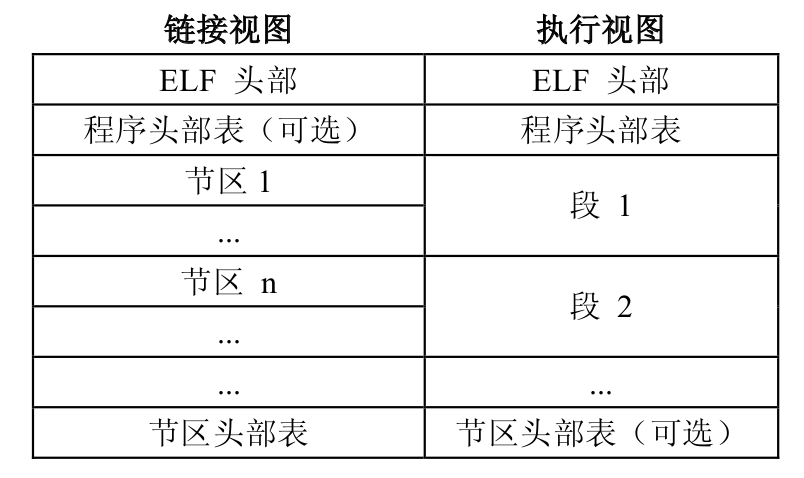
\includegraphics[width=0.55\textwidth]{figure/elf-map.png}
  \caption{链接视图与执行视图}
  \label{elf-map}
\end{figure}

\begin{itemize}
  \item 链接视图
\end{itemize}

在对ELF文件进行链接的过程中,
链接器从链接视图来看待ELF文件,
链接器认为ELF文件被划分为一个个节区(section),
节区中包含代码或者数据。
链接器通过合并这些段来形成新的ELF文件。

\begin{itemize}
  \item 加载视图
\end{itemize}

当加载器对ELF可执行文件执行加载操作时,
它眼中的ELF文件是被划分为了一个个段(segmentation)。
在一个使用分页机制的系统中,
每个段都是按照页大小(例如4KB)进行对齐的。
加载器的任务就是把每个段的页拷贝到主存的合适位置。
(使用虚拟存储器的系统中,加载器不拷贝数据,
只建立虚拟内存和磁盘文件的关联,
在此可以简单认为加载器按照段结构进行了ELF文件到主存的拷贝)

ELF文件中,存在以下的数据结构,来实现链接视图和执行视图。
(在.o文件中,不存在执行视图)

%\begin{itemize}
 % \item ELF头部
%\end{itemize}

\begin{itemize}
  \item ELF文件头部
\end{itemize}

图\ref{header}是一个典型的ELF文件头的内容。
ELF文件头位于ELF文件的起始部分,是两种视图都必要的数据结构。
除了标志该文件是ELF文件及其类型之外,头部最重要的作用
在于标明了以下三点:

\begin{description}
  \item [1]  程序入口点位置
  \item [2]  节区头部表位置和节区的数量
  \item [3]  程序头部表位置和段的数量 
\end{description}

\begin{figure}[h!]
  \centering
  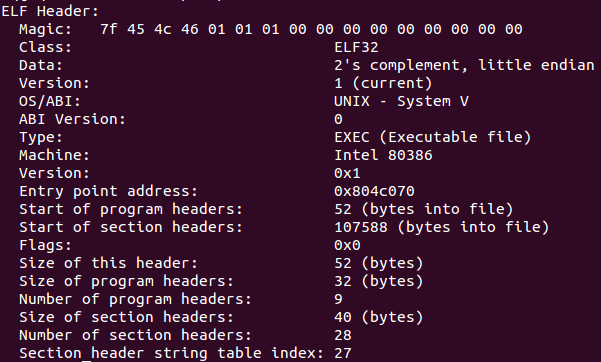
\includegraphics[width=0.5\textwidth]{figure/header.png}
  \caption{ELF文件头部}
  \label{header}
\end{figure}

\begin{itemize}
  \item 节区与节区头部表
\end{itemize}

图\ref{sections}展示了/bin/ls程序的节区头部表的一部分。
在链接视图中,节区用于划分文件中不同类型的数据。
例如.text节用于存放代码,.data节用于存放数据等。
链接两个目标文件的的其中一步,就是把
节区头表为是所有节区的一个索引,
通过解析节区头表可以找到文件的所有节区。

\begin{figure}[h!]
  \centering
  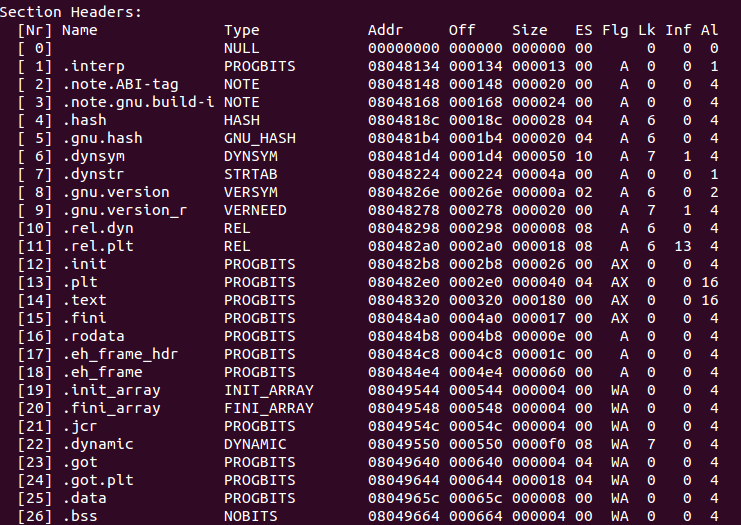
\includegraphics[width=0.5\textwidth]{figure/sections.png}
  \caption{节区头部表}
  \label{sections}
\end{figure}
%\begin{itemize}
 % \item 段和程序头部表
%\end{itemize}

\begin{itemize}
  \item 段和程序头部表
\end{itemize}

图\ref{programs}是/bin/ls的程序头部表。
段是执行视图中的对ELF文件的划分,
ELF文件被加载和执行的就是一个个段。
一般来说,每个节区映射到唯一一个段,而一个段包含不同的节区。
段没有名字,但有类型和属性:
类型一般指明该段是否需要加载至内存,
例如需要加载器加载到主存中的段的类型为“LOAD”;
而段的属性则表明了该段能否被读/写/执行。

\begin{figure}[h!]
  \centering
  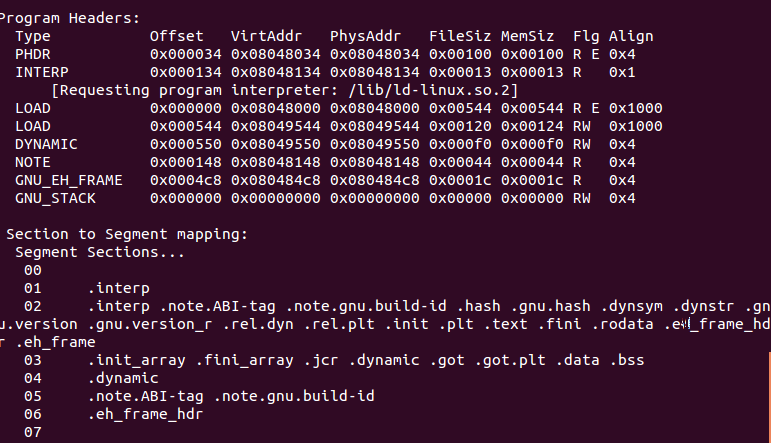
\includegraphics[width=0.5\textwidth]{figure/programs.png}
  \caption{程序头部表}
  \label{programs}
\end{figure}
在一个典型的Linux可执行文件中,
第一个LOAD类型的段一般具有可读和可执行的属性,
该段对应的节区为所有含有代码的节区,例如.init节、.text节和.finit节。

与节区头部表类似,程序头部表是所有段的一个索引。
程序头部表还指明了每个段所包含的节区。


\subsection{文件空间和地址空间}
\label{twoqs}
上文介绍了ELF文件的两种不同的视图,
理解两个视图的区别和联系能帮助我们找到可以插入代码的位置。
然而,这还是不够的。
我们插入的代码必须加载到一定的地址才能被运行。
这就需要理解ELF文件与地址空间的关系。

在节区头部表和程序头部表中,
不但指定了节区或者段在文件中的位置,
还指定了节区或者段在内存中的加载地址。
例如如图\ref{sections}所示,
/bin/ls程序包含的.text节在文件中的偏移是0x3020,
而加载地址为0x8048320。

打个比方,如果在论文中新加入了一个章而没有更新目录,
那么这一章很可能会被读者忽略。
类似地,在ELF文件中插入代码,如果不更新相应的数据结构(节头表和程序头表),
除了增大了文件的体积之外和导致文件不能运行之外,
没有任何意义。

由于插入的代码会影响文件内容在文件中的偏移,
因此相应节头表和段表的偏移字段必须被更新。
如果这项工作没有出现错误,
那么修改后的文件至少是可以正常地像原先一样执行的。
然而,要让我们插入的代码也在加载时被映射到
程序的地址空间中,那插入的部分必须拥有合法的载入地址。

这就带来了两个问题,一是哪些地址空间是空闲并可以使用的,
二是如何让插入的代码刚好使用这部分地址空间。
这两个问题将一直存在于后文对具体技术的讨论中。

第一个问题与操作系统和硬件平台有关,
一个经典的方法是利用段间对齐产生的空间来插入代码。
在一个运行在x86上的Linux系统来说,
由于段的起始地址要按照4KB的页大小进行对齐,
因此加载段之间将会有0~4KB的空余地址空间。
插入的代码可以用于映射到这部分空间。

第二个问题包含很多细节性的修改,
通过小心地把代码插入到一个段的最后,
并修改段的大小,
同时更新后面所有段和节的文件偏移,
就可以让我们的代码刚好用上这一段地址空间。

如果解决了这两个问题,程序再次执行时,插入的代码就已经被加载到
相应的地址空间了。
剩下的问题则会根据需求变化。
例如如何让插入的代码得到执行和在何时执行,
以及如何在插入的代码中使用库函数等。
这些问题将留在具体技术中讨论。

\section{静态链接文件插入技术}

本节将介绍几种典型的、针对静态链接的ELF可执行文件的插入技术。
在前文中,我们讨论了关于文件空间和地址空间的问题,
得出的结论是我们必须兼顾这个方面。
然而在实际的技术中,
要真正向ELF文件中插入代码并使我们的代码运行起来,
特别是能够在代码体中做一些事情,
还需要很多的努力。

\subsection{利用nop指令串插入代码}
\label{nopinjection}

首先介绍一种最简单的代码插入方式。
一本优秀的反汇编教材\cite{heike}中
讲述了利用nop串向ELF文件插入代码的方法。
由于gcc编译器在生成ELF文件时,
会对函数的起始地址按照0x10进行对齐。
多余的空间会使用nop指令(操作码为0x90)进行填充。
由于地址对齐而留下的nop指令串便可以供我们随意使用。

这些可用的nop指令串有这样两个条件:
在nop串第一个nop指令的前面必须是ret或者jmp指令,
而且最后一个nop串之后的地址能够被10h整除。
代码\ref{nop}是/bin/ls文件反汇编之后的一部分代码,
代码中从地址805ac43h开始,到805ac4fh结束的nop指令串
满足上述的两个条件
(前面紧挨的指令为jmp,nop串结束后的地址为805ac50h)。
因此这些nop都可以被改写,
而不影响程序运行。

\begin{lstlisting}[
  language={[x86masm]Assembler},
  caption={/bin/ls中存在的nop指令串},
  label={nop},
]
805ac3e:       5f                  pop    edi
805ac3f:       5d                  pop    ebp
805ac40:       c3                  ret
805ac41:       eb 0d               jmp    805ac50<__sprintf_chk@plt+0x10f90>
805ac43:       90                  nop
805ac44:       90                  nop
805ac45:       90                  nop
805ac46:       90                  nop
805ac47:       90                  nop
805ac48:       90                  nop
805ac49:       90                  nop
805ac4a:       90                  nop
805ac4b:       90                  nop
805ac4c:       90                  nop
805ac4d:       90                  nop
805ac4e:       90                  nop
805ac4f:       90                  nop
805ac50:       f3 c3               repz ret
\end{lstlisting}

虽然这样的nop指令串在/bin/ls这样的文件中有很多,
但每一段都不是太长,容不下很多代码。
一个最简单的办法就是,
在每个nop串快要用完的时候,使用jmp或其他指令,
跳转到下一个nop串的开始处。
这样我们就可以利用几乎所有的nop指令串
(除非有的实在太短,以至于写不下jmp指令)。
\cite{heike}中给出了一个简单的手动修改的示例,劫持一个可执行文件,
在运行它时先打印字符串“hello”。
示例的工作可以归结为以下几个步骤:

(1)修改ELF文件入口点处的两条指令,
替换为jmp指令,跳转地址为第一个nop指令串。

(2)在nop串中写入使用系统调用
打印“hello\textbackslash n”的汇编代码。
如果一个nop串不足,则跳转后继续使用下一个nop串。

(3)打印代码的最后,加入ELF入口点被修改的两条指令。

(4)使用jmp跳转回入口点处的第三条指令。

修改完成后,当我们再次在终端中执行该可执行文件时,
终端中会首先打印出一行“hello”,接着才是它原先的工作。

这种修改方式虽然原理简单,
但若对较大的文件注入大量的代码,
手工操作的工作量会很大。
最好的办法是使用\cite{infelf}提供的infelf工具,
该工具把使用nop进行插入的原理流程化,
从而帮助我们自动完成插入。

Infelf工具在流程上与前面所述差异不大,
但是通过它可以劫持程序执行流的任意的位置,
比如任意一个函数的入口,而不仅限于入口点。
该工具的出现说明向nop串插入代码,
完全可以成为一种常规的插入方式。

然而,如果要插入大量的代码,
程序中仅有的一点nop指令串能够用吗?
我们做一个简单的统计,来看看一个ELF可执行文件中,
大概能留下多少可供使用的nop指令串。
我们选取了一些典型的ELF文件,包括一个最简单的C语言“hello,world!”程序,
若干/bin目录下的实用程序和我们的目标VxWorks镜像。
统计结果如表\ref{nopbytes}所示。

\begin{table}
  \centering
  \caption{典型ELF文件中的nop串占据的空间}
  \label{nopbytes}
  \begin{tabular}{l|l|l}
     \hline
     ELF文件       & 文件大小(字节)& nop串大小(字节) \\ \hline
 “hello,world!”程序  & 7339           & 30                 \\ \hline
     /bin/ls      & 108708          & 921                \\ \hline
     /bin/rm      & 303484         & 1653                \\ \hline  
     /bin/bash    & 924892        & 13723              \\ \hline
     VxWorks系统镜像 & 1337184        & 21114              \\ \hline
  \end{tabular}
\end{table}  

由此可见,随着ELF文件体积的增大,
可用的nop串空间也几乎在正比例扩张,
二者的比例大概维持在100:1的数量级。
除了在最简单的“hello,world!”程序中几乎什么都插不下之外,
具有一些实用功能的应用程序都有着比较可观的空间。
试想一下,假若/bin/bash中13KB的nop串被全部塞满恶意代码,
完全可以对系统产生严重的打击。

\subsection{在代码段的最后分区插入代码}

Silvio Cesare由于在1998年提出的最原始的UNIX病毒模型\upcite{silvio},
而曾被称为“ELF大师(ELF master)”。
在这一病毒模型中,病毒在感染其他文件时,
采取了一种不同的方式。
具体来说是在第一个可加载段(俗称的代码段)最后一节的最后插入代码。
这一方案具有很大的通用性,
因为不论ELF文件有多大,
两个加载段之间都有大概4KB的地址空间供我们插入。
即使总共才只有7KB的“hello,world!”程序也不例外,如图\ref{hello}所示。
第一个LOAD段的结束地址为0x80485b4(0x8048000+0x5b4),
而第二个LOAD段从0x8049f08才开始,
两个段之间有多达0x1954的空闲地址空间。

\begin{figure}[h!]
  \centering
  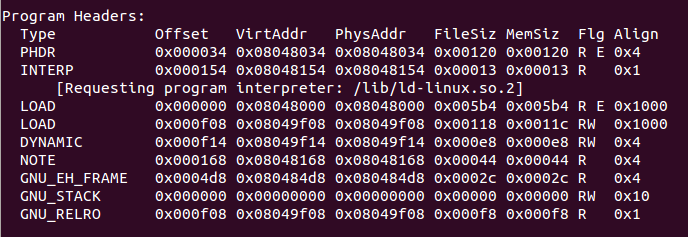
\includegraphics[width=0.5\textwidth]{figure/helloprograms.png}
  \caption{hello程序的程序头部表}
  \label{hello}
\end{figure}
%%

之所以会出现这么大的空闲地址空间,
来源于Linux(包括一些其他的UNIX)的特殊的段加载机制。
因为如果完全按照0x1000来对齐段的起始地址,
将会对物理内存产生巨大的浪费。
从图\ref{hello}可以看出,
hello程序的第一个段只有0x5b4字节大小,
让它完全占有一个物理段,那就会产生0x1000-0x5b4=0xac4字节的浪费,
空间利用率只有35.6\%。


针对这种浪费,Linux的做法是通过分配更多的虚拟内存来
换取物理内存的节约。
具体做法是把可执行文件从偏移0处开始,
按照页大小进行划分,
划分得到的每个页面作为一个物理页面加载。
这样的问题在于有的物理页面会包含两个ELF段,
这时只需要把这样的物理段映射两次到虚拟地址空间即可。
如图\ref{linuxmap},假设一个ELF文件有三个段需要加载,
在使用这种段合并机制的情况下,
三个段之间会产生两段空余的地址空间。

%%%%%%

\begin{figure}[h!]
  \centering
  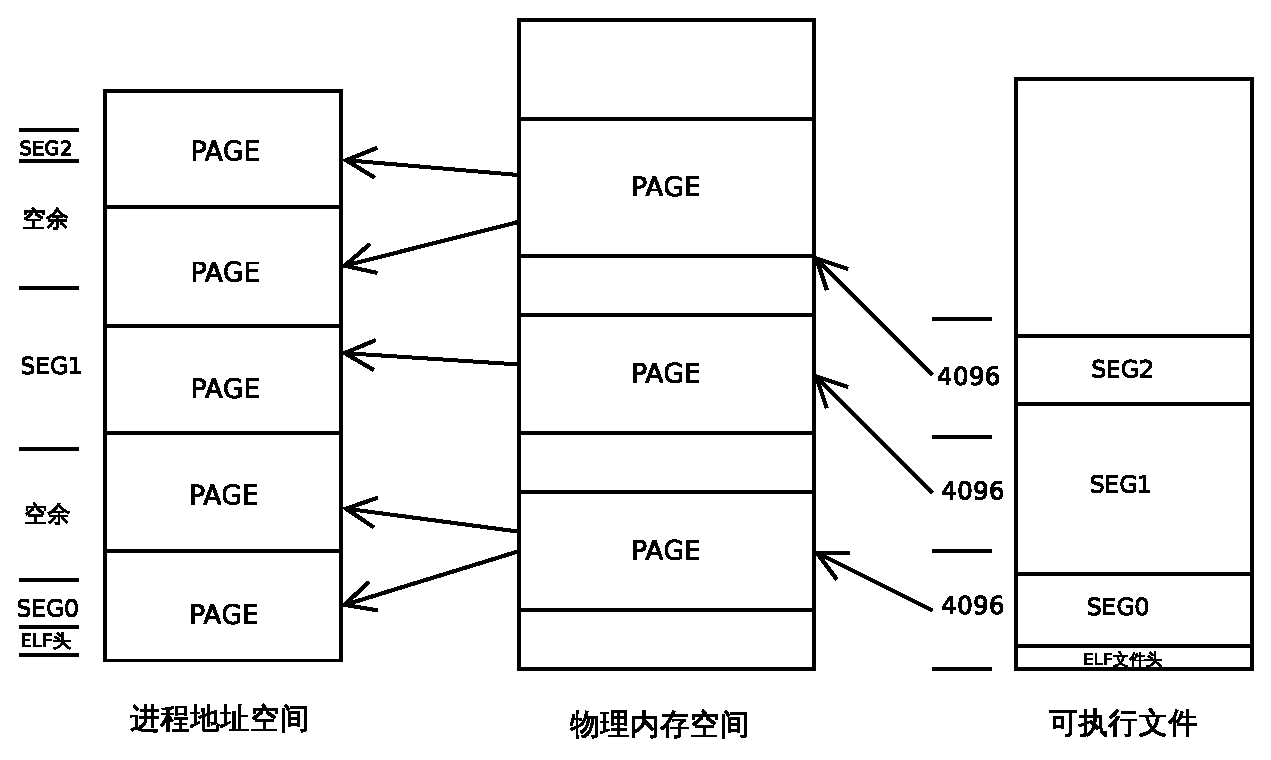
\includegraphics[width=0.8\textwidth]{figure/linuxmap.eps}
  \caption{Linux加载机制中的段合并}
  \label{linuxmap}
\end{figure}



显然,在物理地址空间中,页面利用率大幅提高,
但在虚拟地址空间中留下了尺寸不小的碎片,
图\ref{linuxmap}的情况是碎片大概1页大小,
但在有些gcc的版本中,这一大小甚至接近两个页。
这一空间便可以被我们用于插入代码。
要注意的是,虽然原理上,
数据段最后的剩余空间同样可以利用,
但这需要修改数据段的可写属性,
不如插在代码段之后更为便捷。
因此在\cite{silvio}的算法中,
代码的插入位置是在代码段之后。

下面简要描述了这一插入算法:

1、修改ELF文件头中的entrypoint字段,指向即将插入代码的位置
(代码段offset+filesz)

2、找到ELF中的第一个可加载段(代码段),将该段的filez字段和memsz字段增加
要插入代码的大小。

3、对于所有在代码段之后的段,将其offset增加一页(4KB)的大小。

4、对于代码段的最后一个节区,将其len字段增加插入代码长度大小。

5、对于在代码段之后的所有节区,将其len字段增加一页(4KB)的大小。

6、将插入代码的长度填充到1页(4KB),然后拷贝到预定的插入代码的位置。

7、修改的插入代码,插入一条jmp指令,跳转回原先的entrypoint。

这一算法提出之后,大量的针对ELF乃至Linux内核的研究
都借鉴了其插入代码的思路,
如\cite{simple,prototype,subversive,cerberus,sharelib}。等

在这一算法的基础上,我实现和完善了这一方法的python版本(见附录\ref{python})。
并增加了一些自定义的功能。下面借助一个例子来进一步说明其原理。

这个例子的目标是在一个hello程序中插入代码,
插入代码的任务则是借助Linux的系统调用,
打印一行字符串“foo”。
插入成功的标志是运行hello程序时,先打印一行“foo”,再打印一行“hello”。

图\ref{main1}和\ref{main2}分别展示了在插入代码前后的程序头表的变化。
我们可以很容易在这里发现一些上面的算法所描述的改变,
例如第一个LOAD段的长度被增加了0x26,
而从第二个LOAD段开始,所有的段的偏移量都增加了0x1000,即4K等。
类似地,节区头部表中的一些数据结构也被修改,在此就不再赘述了。

\begin{figure}[h!]
  \label{main}
   \centering
  \begin{tabular}{cc}
    \subfigure[插入前]{
      \label{main1}
      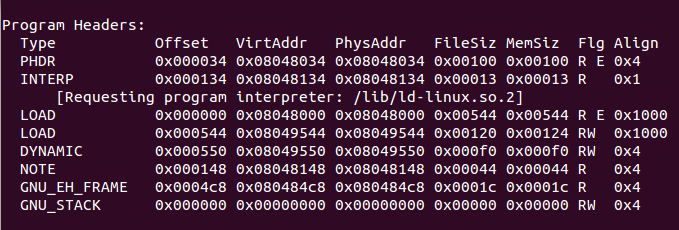
\includegraphics[width=0.6\textwidth]{figure/main.png}
     }  \\
    \subfigure[插入后]
     {
        \label{main2}
      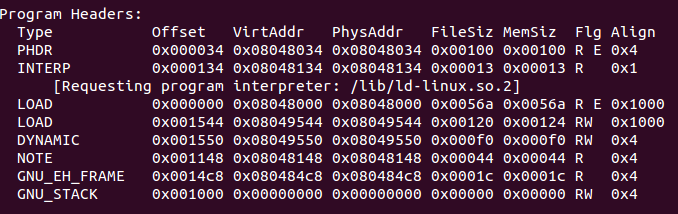
\includegraphics[width=0.6\textwidth]{figure/main2.png}
     }
    \end{tabular}
  \caption{可执行文件插入代码前后的程序头表对比}
\end{figure}
          
图\ref{dia}展示了插入的代码如何通过修改程序入口点
对程序原有的正常执行流进行篡改。
在程序未被修改前,
ELF头的入口点指向代码段的起始位置,如图\ref{dia1}。
通过修改ELF头的入口点,
使它指向我们插入代码的位置;
在插入代码的最后,跳转回原入口点的位置,
以保证程序的正常执行,如图\ref{dia2}。

\begin{figure}[h!]
   \centering
  \begin{tabular}{cc}
    \subfigure[插入前]{
      \label{dia1}
      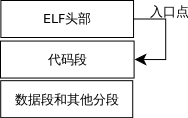
\includegraphics[width=0.3\textwidth]{figure/dia1.png}
     }  
    \hspace{4em}
    \subfigure[插入后]
     {
        \label{dia2}
      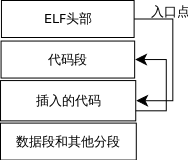
\includegraphics[width=0.3\textwidth]{figure/dia2.png}
     }
    \end{tabular}
  \caption{可执行文件代码插入前后执行流程对比}
  \label{dia}
\end{figure}


\subsection{在代码段之前插入代码}

虽然利用代码段最后可能空余的地址空间来插入代码,
已经成为了一种比较成熟的手段,
但这种方法的局限性仍然是不可忽视的。
最重要的一点就是其插入的代码量存在限制。
一般来说,如果插入代码量最好保证在1KB之内,
一旦超过2KB,几乎是不可能成功的。

然而,一个高效而便捷的工具ELFsh\upcite{elfsh}
提供了一种新的插入思路,
即把代码插入至代码段之前。
我们知道,对于一个运行在IA32上的Linux系统来说,
一个进程的地址空间中,代码段总是开始于0x8048000,
然而从0到0x8047fff这段空间一般不被使用。
该工具的思路就是把需要执行的代码插入至
这一段未被使用的地址空间中。

ELFsh工具功能强大,
它以一个.o文件和一个可执行文件作为输入。
不但能够讲.o中的可执行代码插入至可执行文件中,
还能插入.o文件携带的数据节、bss节和符号表。
并能够对插入代码的所有重定位入口进行重定位。

下面简要说明其插入流程:

1、将.o文件的.bss节插入合并到可执行文件的.bss节中。

2、遍历.o文件的所有节区,判断是否具有以下条件
\begin{itemize}
  \item 存在标志位(说明该节区需要被加载到进程空间中)
  \item 在文件中占据空间(排除.bss节区)
  \item 节区类型为值为SHT\_PROGBITS,说明该节区为程序节或者代码节。
\end{itemize}
  
对于同时满足这些条件的节区,再判断节区是否具有可写属性,
对于具有可写属性的节区(数据节),插入到.bss节之后;
其他节区插入到第一个节区之前。

3、把.o文件的符号表合并至可执行文件中。

4、对于.o文件中的所有节区,如果已经被
插入到了可执行文件中,并且需要重定位,
则对其进行重定位。

下面演示ELFsh工具的效果。
我们的目标是劫持/bin目录下的ls程序。
我们首先编写一个简单的程序,
源代码见\ref{myprintf.c},
然后把它编译为myprintf.o即可。
我们的目标是把它注入到ls程序中。
每次运行ls,都会先打印一行“hi, you're hijacked!”。

\begin{lstlisting}[
  language={C},
  caption={myprintf.c源代码},
  label={myprintf.c},
]
#include<stdio.h>
void myprintf(){
    printf("hi, you're hijacked!");
}
\end{lstlisting}

图\ref{fig-matrix}反映了ls程序被插入前后的节头表(只展示了前20个)
和程序头表的变化。
由图可以发现,在ELFsh向可执行文件注入了9个节区,
并都位于可执行文件的第一个节区,即.interp节之前。
(此外还进行了符号表和.bss节的合并,这里看不出来)。
程序头表方面,可以发现段的数目并没有变化,
但是第一个段的起始地址由0x8048000提前到了0x803c000,
这也说明注入的代码使用了0x8048000之前的地址空间。
此外,位于后面的段在文件中的偏移也相应地增加了0xc000,
说明我们在.interp段之前总共插入了0xc000字节的代码,
即12个页,
试想一下,如果使用nop插入或者插入到段间的空闲地址,
这几乎是不可能完成的任务。

\begin{figure}[h!]
    \centering
    \begin{tabular}{cc}
        \subfigure[插入前节头表]{
            \label{fig-matrix-a}
            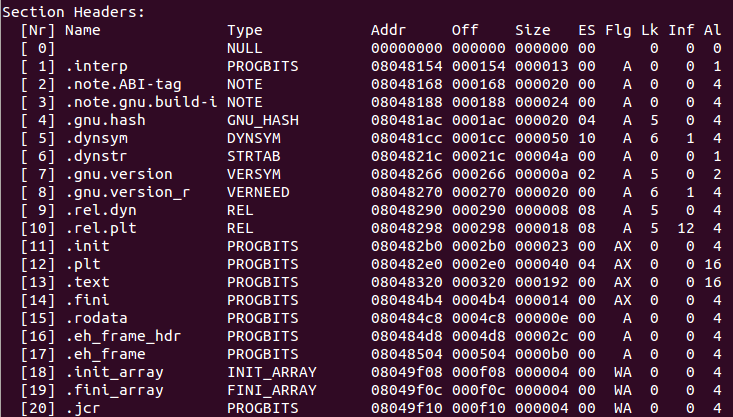
\includegraphics[width=.46\textwidth]{figure/sht1.png}
        } \hspace{2em} &
        \subfigure[插入前程序头表]{
            \label{fig-matrix-b}
            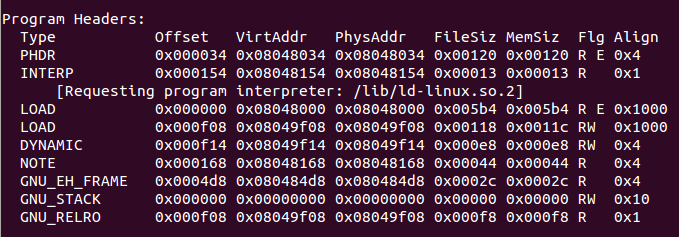
\includegraphics[width=.38\textwidth]{figure/pht1.png}
        } \\
        \subfigure[插入后节头表]{
            \label{fig-matrix-c}
            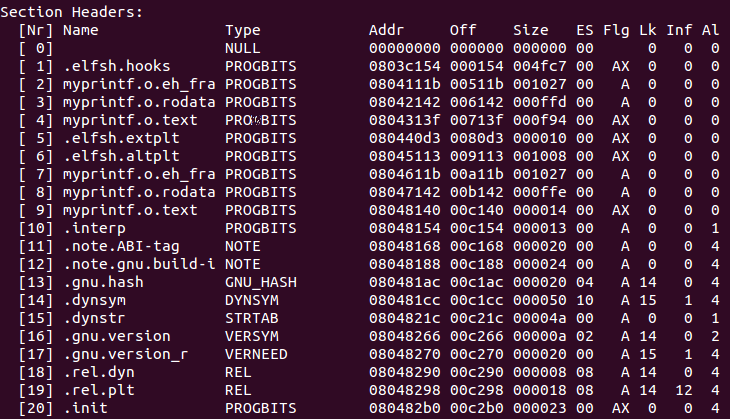
\includegraphics[width=.46\textwidth]{figure/sht2.png}
        } \hspace{2em} &
        \subfigure[插入后程序头表]{
            \label{fig-matrix-d}
            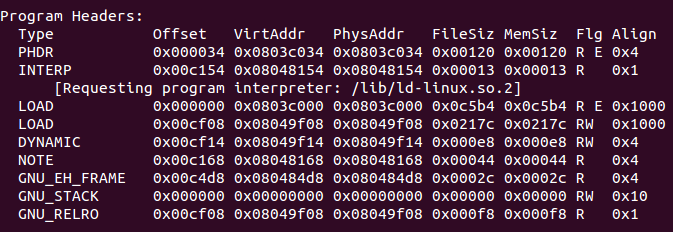
\includegraphics[width=.38\textwidth]{figure/pht2.png}
        }\\
    \end{tabular}
    \caption{插入前后ls程序头表和节头表变化}
    \label{fig-matrix}
\end{figure}

插入一旦完成,劫持工作就会很容易进行。
我们只需要手动修改ELF文件的入口点,
指向myprintf函数的地址,然后手动修改该函数的最后几条指令,
跳回原入口点即可
(回想一下,函数结尾往往有nop指令串,因此这很容易实现)。

最后的达到的效果如图\ref{ls}所示。

\begin{figure}[h!]
    \centering
    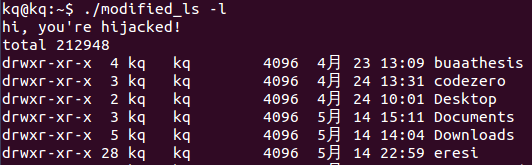
\includegraphics[width=.6\textwidth]{figure/ls.png}
    \caption{修改后的ls程序运行结果}
    \label{ls}
\end{figure}

\section{动态链接文件劫持技术}

Linux下的大部分程序都使用动态链接。
动态链接的程序对外部库函数的调用,
需要通过got(Global Offset Table,全局偏移表)和
plt两个数据结构间接进行。
这在某种程度上为我们劫持这些库函数外部库函数
提供了方便。
因为我们可以利用这一层中转,
通过篡改got和plt来劫持函数调用,
而不需要直接修改代码部分中的地址或者在被劫持函数中增加跳转。

\subsection{利用修改共享库地址和名称进行劫持}

ELF中文件关于动态链接的细节,
应参见\cite{elf1.2},
然而,本条中讲述的劫持方法,
不但简单明了,而且像教科书一般阐明了ELF中
对动态库函数的引用机制。

我们的目标仍然是劫持/bin/ls程序,这一次我们不修改
任何程序中的代码,包括nop指令串,
而仅仅是修改文件中一个与动态链接
有关的数据结构,即.dynamic节。
就可以实现对它的劫持。
\begin{figure}[h!]
    \centering
    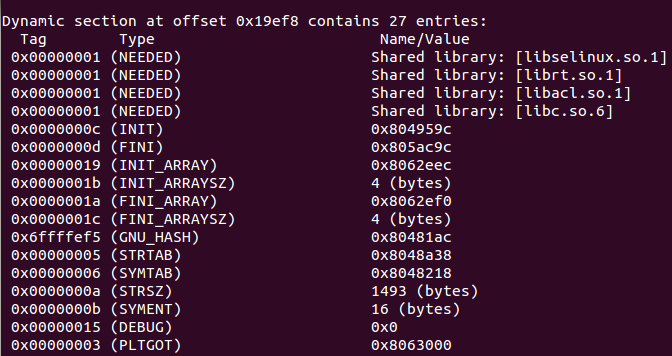
\includegraphics[width=.6\textwidth]{figure/lsdyn1.png}
    \caption{ls程序的.dynamic节}
    \label{lsdyn1}
\end{figure}

ls程序的.dynamic节如图\ref{lsdyn1}所示。
类型为“NEEDED”的入口指明了该程序所依赖的共享对象,
这些共享对象默认位于/lib目录下。
如果我们能够在这里面加一个条目,
填上我们自己编写的共享对象名称,
那程序运行过程中,是否就会链接到我们自己的共享对象,
甚至引用我们自己编写的函数呢?
答案是肯定的。



由于ls函数每次运行,
都会调用动态C库(libc.so.6)中的一些函数,
例如opendir()函数。
假设我们的目标是劫持这个函数,
我们只需要自行编写一个同名函数,
并编译为一个共享对象,
例如rt.so.1,放在/lib下。
rt.so.1的源代码见代码\ref{rt},
其中使用了显式运行时链接技术,
即在函数体中显式地调用“原版”的opendir()函数。

\begin{lstlisting}[
  language={C},
  caption={rt.so.1源代码},
  label={rt},
]
#include <stdio.h>
#include <sys/types.h>
#include <stdlib.h>
#include <fcntl.h>
#include <dirent.h>
#include <dlfcn.h>

#define LIBC_PATH    "/lib/i386-linux-gnu/libc.so.6"

DIR     *opendir(const char *name)
{
   void  *handle;
   void  *(*sym)(const char *name);

   handle = dlopen(LIBC_PATH, RTLD_LAZY);
   sym = (void *) dlsym(handle, "opendir");
   printf("hi, you're hijacked!"); 
   return (sym(name));
}
\end{lstlisting}

下面我们要做的是让ls程序执行时调用自己编写的
opendir(),而不是调用libc.so.6中的原版函数。
我们注意到.dynamic节中有一个入口的类型为“DEBUG”,
这个入口在程序实际运行中并没有实际作用。
因此我们把它的值和类型修改为与第二个条目相同。
然后把第二个类型为NEEDED条目的的值改为"rt.so.1"即可。
修改结果如图\ref{lsdyn2}所示。

\begin{figure}[h!]
    \centering
    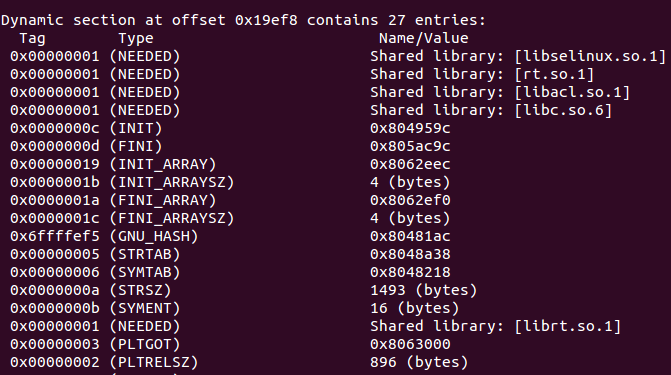
\includegraphics[width=.6\textwidth]{figure/lsdyn2.png}
    \caption{修改后的ls程序的.dynamic节}
    \label{lsdyn2}
\end{figure}

这样一来,ls在动态链接过程中,
就会将我们自己编写的rt.so.1链接进来。
并且由于在.dynamic节中,
rt.so.1位于libc.so.6之前,
因此在动态链接器的符号解析过程中,
因此我们编写的opendir()将会取代原版的函数,
因此在执行中,被调用的是我们编写的opendir()函数。
修改完成后,我们可以得到与图\ref{ls}类似的结果。

\subsection{利用修改plt和got进行劫持}
\label{plt+got}
上一条介绍的动态链接库劫持技术,
看似非常简单,但实际应用中,
可能有不少的限制,比如:

\begin{itemize}
  \item 可执行文件的.dynamic节不存在“DEBUG”入口
  \item 没有足够的权限向/lib下添加动态库文件
  \item 自行编写的库函数不能找到原版的库函数 
\end{itemize}

以上任何一点都会导致这种方法变得无比复杂,最后失败。
本条我们回归原始的物理插入方式,
看看能否通过插入代码来实现劫持。

劫持动态库函数的调用,
需要我们插入两段代码:
A段在函数入口点处执行,作用是帮助我们修改got,
定位到插入库函数的位置。
B段则是我们插入的库函数。
这两段代码的插入可以用上一节中描述的三种方法
的任意一中来进行。

两段代码的算法简要描述如下:

A:

1、使用系统调用,为代码段增加可写属性。

2、保存got中对应条目的地址,记为original\_got。

3、将got中条目的地址修改为插入的库函数的地址。

B:

1、执行目的操作,例如打印一行信息。

2、恢复got中旧的条目的地址。

3、恢复堆栈,调用原库函数。

4、保存got中的地址,覆盖original\_got。

5、将got中的地址替换为插入的库函数的地址。

在B代码的第4步要重新保存一遍original\_got,
因为动态链接程序大都是用“延迟绑定”机制,
在第一次调用库函数时,
会经过plt进行一次间接跳转,
并会调用动态链接器进行重定位,
从而修改got中保存的地址。


\section{ELF文件插入技术总结}

至此,我们已经介绍了5种对ELF文件进行插入的技术,
包括三种针对静态编译程序的物理插入方法,
和两种劫持动态链接程序的方法。
本节对上述的方法进行总结和补充。

表\ref{conclusion1}首先对展示了
三种静态ELF文件的插入技术的对比情况。

\begin{table}
  \centering
  \caption{ELF代码插入技术对比}
  \label{conclusion1}
  \begin{tabular}{l|l|l|l}
     \hline
     插入技术  & 利用nop指令串 & 插入到代码段之后&插入到代码段之前 \\\hline \hline
 可插入代码量  & 约为文件大小的1/100  & 少于1KB & 大于100KB   \\ \hline
   劫持位置    &  本地   &   本地 & 本地            \\ \hline
  编写插入代码的语言 & 汇编语言 & 汇编语言 & C语言  \\ \hline
   插入代码调用外部函数& 手动寻址  & 手动寻址 & 自动重定位       \\ \hline  
     局限性  & 插入代码量依赖文件大小&插入代码量小于1KB& -       \\ \hline
  \end{tabular}
\end{table} 

表\ref{conclusion2}展示了两种动态劫持机制的对比情况。

\begin{table}
  \centering
  \caption{动态链接文件劫持技术对比}
  \label{conclusion2}
  \begin{tabular}{l|l|l}
     \hline
     劫持技术  & 通过修改.dynamic结构&通过修改got   \\\hline \hline
 可插入代码量  & 不限  & 与使用的代码插入技术相关   \\ \hline
   劫持位置    & 外部库函数 & 外部库函数            \\ \hline
  编写插入代码的语言 & C语言 & 汇编语言         \\ \hline
   插入代码调用外部函数 & 自动重定位  & 手动寻址       \\ \hline  
     局限性  & 见\ref{plt+got} & 较为繁琐,移植性差       \\ \hline
  \end{tabular}
\end{table} 

 



%\section{ELF插入技术在vxWorks中的使用分析}

%%
%%\section{C\TeX{}套装 [Windows Only]}
%%
%%C\TeX{}套装是Windows下为中文优化的\LaTeX{}系统套件,主要基于MiKTeX系统,
%%集成了编辑器WinEdt和其他相关软件。整个系统封装在一个安装程序中,
%%安装方法与常规软件相同,无需任何配置,适合大部分Windows用户使用。
%%
%%\begin{description}
%%    \item[下载地址] \hfill
%%    \begin{description}
%%        \item[官方页面]
%%            \url{http://www.ctex.org/CTeXDownload}
%%        \item[未来花园]
%%            稍后我们也会提供未来花园上的下载页面,敬请关注
%%    \end{description}
%%    \item[安装方法] \hfill
%%        \begin{itemize}
%%            \item[] 与常规软件的安装方法差不多
%%            \item[] 一直下一步稍加一些自定义(如安装路径)即可
%%        \end{itemize}
%%\end{description}
%%
%%\section{\TeX{}Live [ Windows \& Linux ]}
%%
%%\TeX{}是自由软件,有很多发行版本,就像Linux的Ubuntu、Fedora等等。
%%每个发行版本都是一套工具集合,包括plain\TeX{},\LaTeX{},pdf\TeX{},dvips等。
%%其中比较流行的是\TeX{}Live,也包含在CTAN的开源镜像中,
%%目前的最新版本是\TeX{}Live 2012。
%%
%%推荐通过下载ISO镜像文件的方式安装:
%%\begin{description}
%%    \item[官方说明]
%%        \url{http://www.tug.org/texlive/acquire-iso.html}
%%    \item[下载地址] 官方地址会自动跳转寻找"最近"镜像,还有几个较快的教育网镜像
%%    \begin{description}
%%        \item[官方地址]
%%            \url{http://mirror.ctan.org/systems/texlive/Images/texlive2012.iso}
%%        \item[清华镜像]
%%            \url{http://mirrors.tuna.tsinghua.edu.cn/CTAN/systems/texlive/Images/}
%%        \item[北交镜像]
%%            \url{http://mirror.bjtu.edu.cn/CTAN/systems/texlive/Images/}
%%        \item[未来花园]
%%            稍后我们也会提供未来花园上的下载页面,敬请关注
%%    \end{description}
%%    \item[安装方法] \hfill
%%    \begin{enumerate}
%%        \item 通过虚拟光驱挂载镜像也可以直接打开或解压缩不过会比较慢
%%        \item 双击运行光盘镜像或者运行脚本
%%        \item[] Windows 用户可以直接双击运行\textsl{install-tl.bat}
%%        \item[] Linux 用户可以在终端下执行命令\textsl{./install-tl}
%%        \item 按照提示下一步即可,安装大致耗时10$\sim$20分钟,受机器配置影响。
%%    \end{enumerate}
%%\end{description}
%%
%%当然官方也提供了通过网络安装的方式,虽然通过可以通过镜像选择达到比较快的速度,
%%但是这里简便期间不再赘述,有兴趣的同学可以参考官方说明
%%\url{http://www.tug.org/texlive/acquire-netinstall.html}。
%%
%%\section{Mac\TeX{} [ Mac ]}
%%
%%Mac\TeX{}是基于\TeX{}Live为Mac系统设计的套件。
%%
%%\begin{description}
%%    \item[官方网站]
%%        \url{http://tug.org/mactex/}
%%    \item[下载地址] 官方地址会自动跳转寻找"最近"镜像,还有几个较快的教育网镜像
%%    \begin{description}
%%        \item[官方地址]
%%            \url{http://mirror.ctan.org/systems/mac/mactex/MacTeX.pkg}
%%        \item[清华镜像]
%%            \url{http://mirrors.tuna.tsinghua.edu.cn/CTAN/systems/mac/mactex/}
%%        \item[北交镜像]
%%            \url{http://mirror.bjtu.edu.cn/CTAN/systems/mac/mactex/}
%%        \item[未来花园]
%%            稍后我们也会提供未来花园上的下载页面,敬请关注
%%    \end{description}
%%    \item[安装方法] 同一般软件安装,下一步即可
%%\end{description}
%%
%%\section{关于编辑器}
%%
%%以上介绍了三款\LaTeX{}套装,涵盖了主流的三大平台,除了C\TeX{}自带了WinEdt,
%%其余两款均需要自己选择编辑器,理论上任何文本编辑器都是可以使用的,
%%如Windows上的Notepad++,Linux/MacOS上的vim,emacs,
%%一方面要考虑对\LaTeX{}的支持,一方面还是自己的熟悉程度。
%%
%%这里推荐一款大众化的编辑器\TeX{}maker,它是跨平台的,支持Windows、Linux和MacOS。
%%
%%\begin{description}
%%    \item[官方网站]
%%        \url{http://www.xm1math.net/texmaker/}
%%    \item[下载地址]
%%        \url{http://www.xm1math.net/texmaker/download.html}
%%    \item[相关说明]
%%    \begin{itemize}
%%        \item 安装同一般软件的安装
%%        \item 配置Xe\LaTeX{}的编译,选择菜单栏“选项”->“配置\TeX{}Maker”,
%%        \item[] 在“\LaTeX{}”一栏填写
%%            \texttt{xelatex -interaction=nonstopmode\%.tex}
%%    \end{itemize}
%%\end{description}
%%
%%\section{关于编译}
%%
%%\LaTeX{}的文件是通过编译生成的,对于本模板和毕业设计论文而言,
%%需要经过代码\ref{code-compile}所示步骤(以sample-bachelor.tex为例):
%%\begin{lstlisting}[
%%    language={bash},
%%    caption={编译步骤},
%%    label={code-compile},
%%]
%%xelatex sample-bachelor.tex
%%bibtex  sample-bachelor.aux
%%xelatex sample-bachelor.tex
%%xelatex sample-bachelor.tex
%%\end{lstlisting}
%%当然,我们在模板里也提供了编译的执行脚本。
%%
%%\subsection{批处理 [ Windows only ]}
%%
%%进入cmd(Win+R,然后输入cmd),cd到BUAAthesis对应目录,
%%如{\verb D:\BUAAthesis\ },然后运行{\verb msmake }即可。
%%
%%\subsection{Makefile [ Windows(cygwin) / Linux / MacOS ]}
%%需要要你的命令行环境支持Make,cd到BUAAthesis相应目录,
%%目前支持如代码\ref{code-make}所示的功能:
%%\begin{lstlisting}[
%%    language={bash},
%%    caption={make 命令},
%%    label={code-make},
%%]
%%make bachelor # 编译本科生的\LaTeX{}(文件默认项,亦可直接输入make)
%%make master # 编译研究生的\LaTeX{}文件
%%make clean # 删除编译过程中生成的文件(除了pdf)
%%make depclean # 删除编译过程中生成的文件(包括pdf)
%%\end{lstlisting}
